\chapter{Introdução}

	O cenário atual de comércio em um mundo intrinsecamente globalizado requer eficiência em troca de informações, serviços e mercadorias; ou seja, eficiência logística. A logística é a essência do comércio \cite{ballou2006cadeiasuprimentos}, ela contribui para que pessoas não mais sejam obrigadas a viver perto das fontes de produção e possam trocar mercadorias com outras regiões de forma efetiva, contribuindo decisivamente para melhorar o padrão econômico de vida geral. 
	
	A logística é o processo de planejamento, implantação e controle do fluxo eficiente e eficaz de mercadorias, serviços e das informações relativas desde o ponto de origem até o ponto de consumo com o propósito de atender as exigências dos clientes \cite{cscmp2013supplychainglossary}. Essa definição sugere a logística como um processo, o que significa que inclui todas as atividades importantes para a disponibilização de bens e serviços aos consumidores quando e onde estes quiserem adquiri-los \cite{ballou2006cadeiasuprimentos}.
	
	A cadeia de suprimentos (CS), por outro lado, é um conceito mais amplo. A CS é onde a logística é exercida. São as partes necessárias para se dar suporte ao pedido de um cliente, desde o produtor até o consumidor final. A gestão da cadeia de suprimentos tem como alvo a orquestração de todas as partes envolvidas por meio de uma logística integrada de forma a se otimizar ao máximo o processo de fornecimento de um produto, serviço ou informação.
	
	A ideia de uma CS simples envolve fornecedor, produtor e cliente \cite{hugos2018supplychain}, porém conceitos modernos ampliam a noção de CS para uma cadeia de suprimentos estendida, que inclui diversos outros fornecedores de serviços em áreas como logística, finanças, \textit{marketing} e desenvolvimento; que, mediante coordenação e colaboração, criam oportunidades para melhoria dos custos ou serviços ao consumidor. A Figura \ref{fig:cadeia-de-suprimentos} exemplifica a inter-relação das partes em uma cadeia de suprimentos estendida.
	
	\begin{figure}[H]
		\centering
		\caption{Exemplo de cadeia de suprimentos estendida.}
		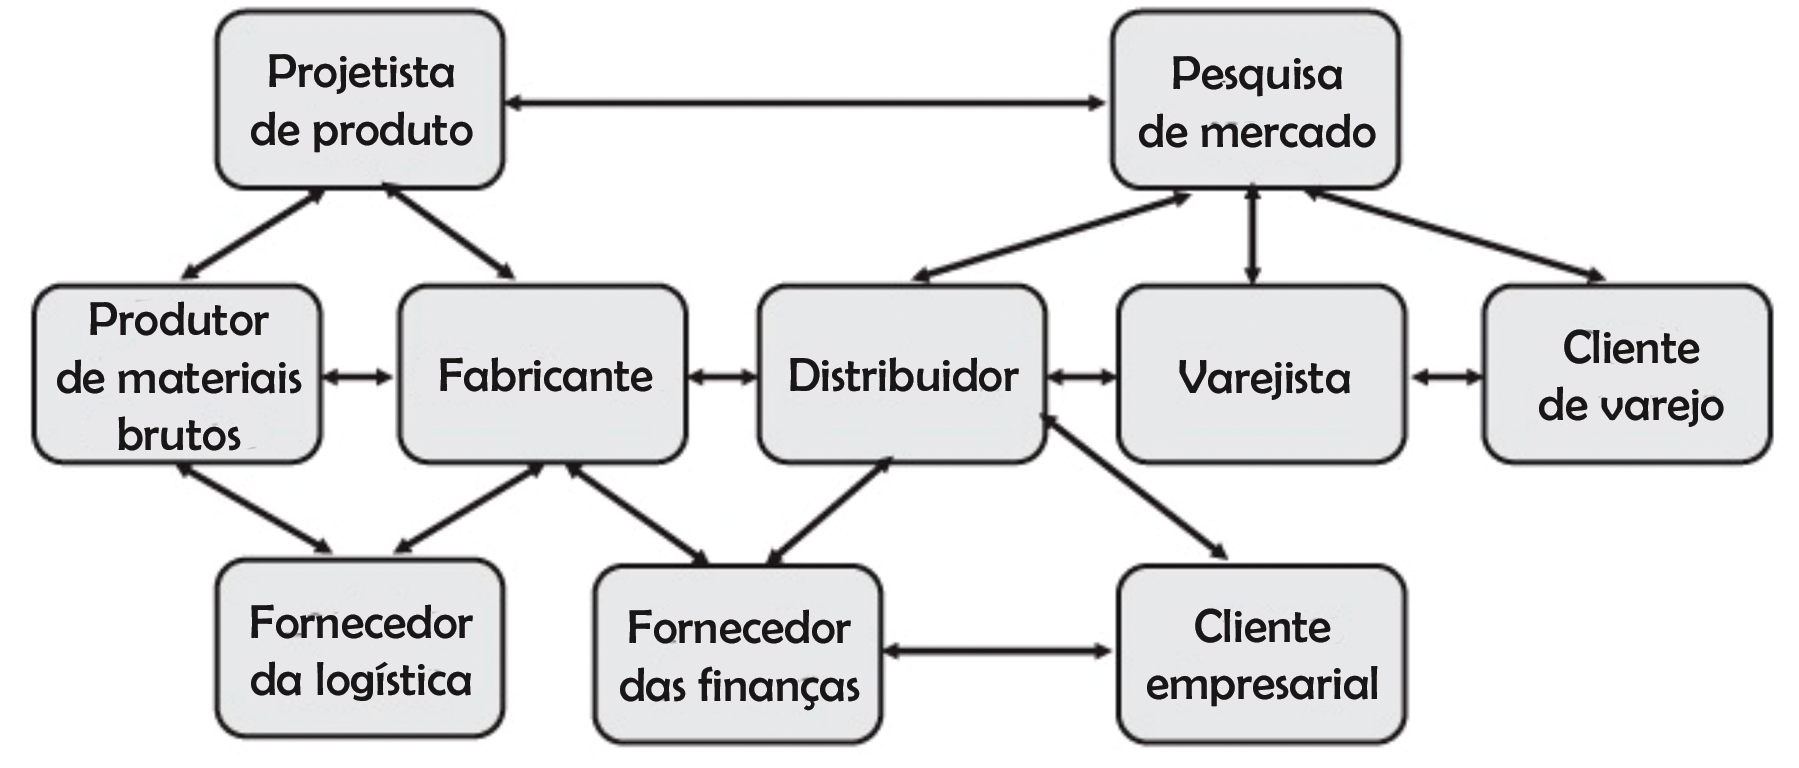
\includegraphics[width=1\textwidth]{cadeia-de-suprimentos.png}
		\label{fig:cadeia-de-suprimentos}
		\source{\citeonline{hugos2018supplychain} (adaptado).}
	\end{figure}

	Além do eficiente fluxo de materiais e produtos dentro da CS, é imprescindível a manutenção de um canal para troca de informações entre as partes em uma CS, pois sem uma adequada comunicação, gerentes podem acidentalmente tomar decisões supostamente racionais, porém que afetam negativamente outros líderes da cadeia, como o efeito chicote \cite{lee1997bullwhip}, que é a distorção da percepção da procura de um produto que vai se ampliando ao longo da cadeia de suprimentos. Erros de comunicação desse tipo podem acarretar problemas como o aumento do custo de transporte, o elevado tempo de aprovisionamento ao cliente e o desgaste no relacionamento com os fornecedores.
	
	Ao longo da cadeia de suprimentos pode-se observar processos que agregam valor ao produto em desenvolvimento. As etapas de transformação do produto com adição de valor ao longo da CS também podem ser definidas como cadeia de valor.
	
	Uma cadeia de valor (CV) é um conjunto de atividades que empresas de um setor específico desempenham a fim de entregar um produto ou serviço que tenha algum valor perceptível para o mercado \cite{porter1985competitiveadvantage}. A ideia da CV é baseada na agregação de valor ao produto a cada processo de transformação ocorrido, processo esse que envolve a aquisição e consumo de recursos (mão de obra, materiais, equipamentos, instalações, administração, etc). \citeonline{porter1985competitiveadvantage} classifica a CV em duas categorias de atividades que agregam valor ao produto: as atividades primárias e as atividades de apoio (vide Figura \ref{fig:porter-cadeia-de-valor}).
	
	\begin{figure}[H]
		\centering
		\caption{Cadeia de valor de Porter.}
		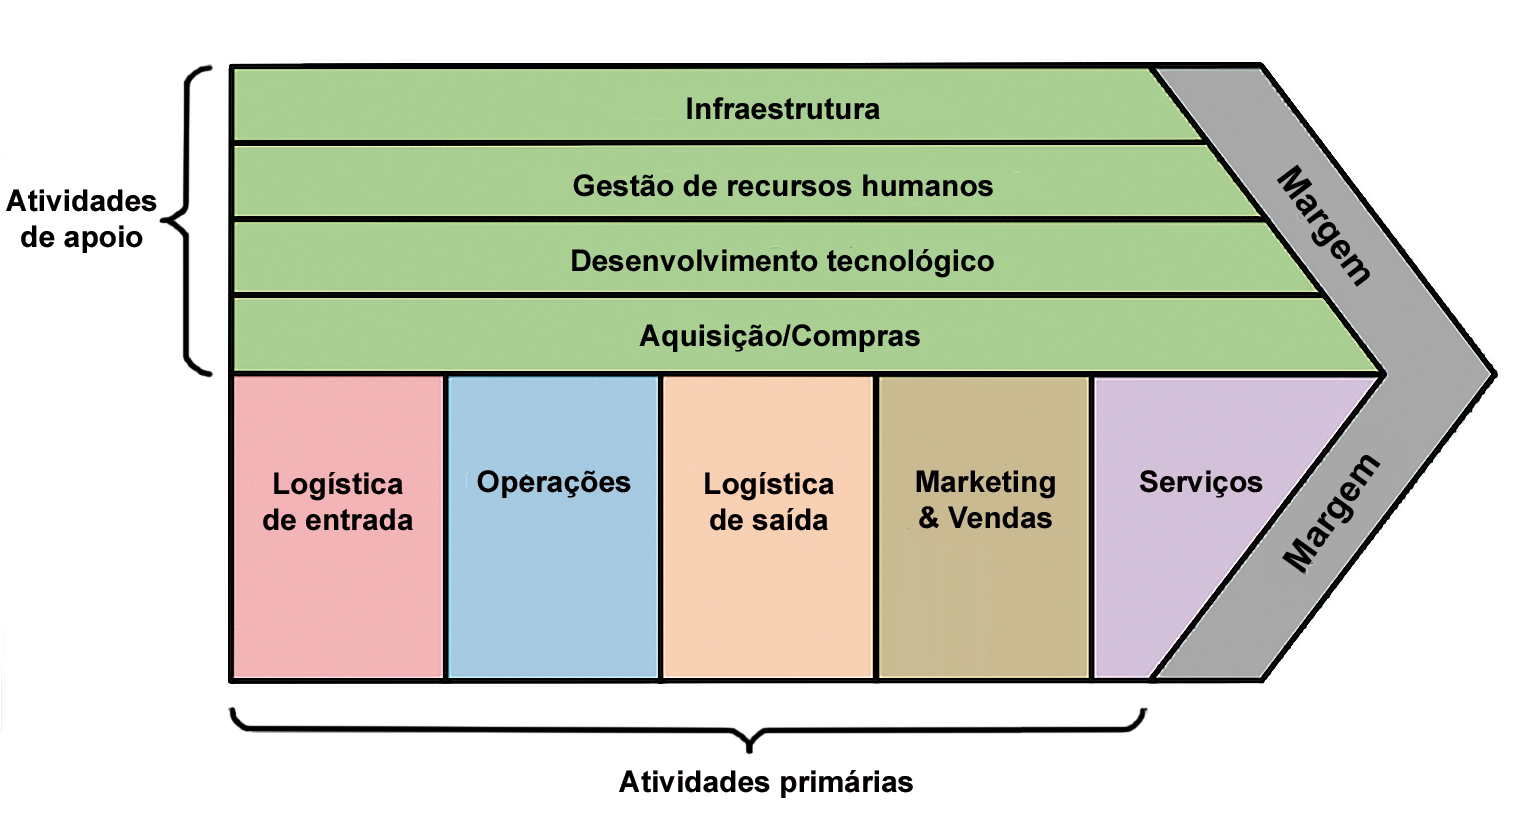
\includegraphics[width=1\textwidth]{porter-cadeia-de-valor.png}
		\label{fig:porter-cadeia-de-valor}
		\source{\citeonline{porter1985competitiveadvantage} (adaptado).}
	\end{figure}
	
	
	As CVs estão focadas em fornecer o máximo valor ao cliente (valor perceptível) com o menor custo e, portanto, é um indicador para a competitividade da empresa. Com o crescente acirramento da competição entre as empresas, essas devem procurar novas formas de agregar mais valor perceptível aos seus produtos, sendo isto em forma de redução de preço, aumento de qualidade, suporte ou qualquer outra nova funcionalidade.
	
	Outra forma de agregação de valor está no princípio de valor compartilhado, que envolve a geração de valor econômico de forma a criar também valor para a sociedade como um todo \cite{porter2011valorcompartilhado} com o enfrentamento de suas necessidades e desafios. Esta necessidade de valor compartilhado parte da percepção generalizada de que empresas prosperam às custas da depreciação da comunidade que as cercam. Soluções que visem o aumento das condições de trabalho, a maior racionalidade e eficiência no tratamento dos recursos naturais necessários para sua atividade e outras formas de balancear o \textit{trade-off} entre eficiência econômica e progresso social são estratégias para se recuperar a legitimidade e a percepção de valor pela sociedade da atividade empresarial.
	
	Atrelado à cadeia de suprimentos e à cadeia de valor existe o conceito de ciclo de vida do produto, que foi um conceito elaborado em meados da década de 1960 com o propósito de criar um modelo que fosse capaz de explicar o sucesso ou fracasso de um produto introduzido ao mercado, sendo capaz também de identificar momentos certos para modificar estratégias de preço, fabricação e quando o produto deve ser descontinuado \cite{cao2012lifecycle}. O modelo inicialmente desenvolvido por \citeonline{levitt1965lifecycle} mostra o padrão de produtos na história passando por quatro estágios bem definidos: desenvolvimento de mercado, crescimento, maturidade e declínio, conforme observado na Figura \ref{fig:product-life-cycle}.
	
	\begin{figure}[H]
		\centering
		\caption{Estágios do ciclo de vida do produto.}
		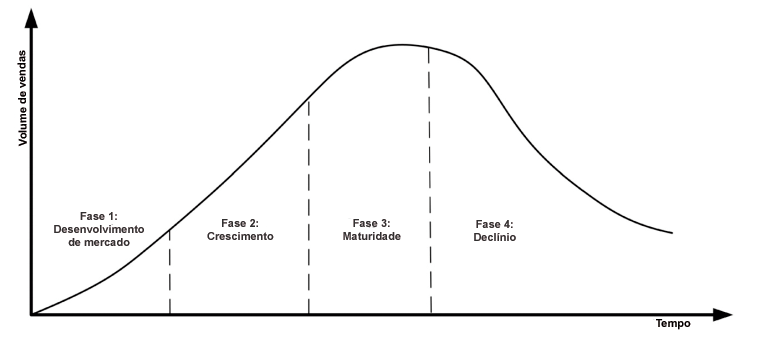
\includegraphics[width=1\textwidth]{product-life-cycle.png}
		\label{fig:product-life-cycle}
		\source{\citeonline{levitt1965lifecycle} (adaptado).}
	\end{figure}

	Vista a tendência global de redução do ciclo de vida do produto devida a rápida taxa de introdução de novas tecnologias para satisfazer a demanda dos clientes, especialmente no mercado de produtos eletrônicos \cite{trappey2008lifecycle}, novas versões de modelos de ciclo de vida do produto vêm sendo elaboradas considerando outros aspectos de mercado e não somente sob a visão da área de \textit{Marketing}. Por vezes, estudos recentes envolvendo ciclo de vida são denominados ``engenharia do ciclo de vida do produto'' (E-CVP) \cite{cao2012lifecycle} e levam em consideração fatores não abordados nos modelos originais como, por exemplo, a fase de pesquisa e desenvolvimento, a retroalimentação de dados, assim como o descarte e reciclagem do produto. Sempre tendo como objetivo auxiliar na tomada de decisões para o sucesso de um produto no mercado.
	
	A Figura \ref{fig:life-cycle-extension} mostra um modelo de ciclo de vida do produto com elementos que incluem a fase de desenvolvimento e a renovação do produto. A renovação do produto e a decorrente extensão de sua vida é essencial, pois mantém o produto no mercado na forma de novas versões e, assim, amplia as receitas mediante ações estratégicas para agregação de valor. O modelo do ciclo de vida e os elementos presentes sempre irão variar conforme a natureza do produto e tipo de mercado consumidor onde o mesmo está inserido.
	
	\begin{figure}[H]
		\centering
		\caption{Modelo de ciclo de vida do produto com renovação do produto.}
		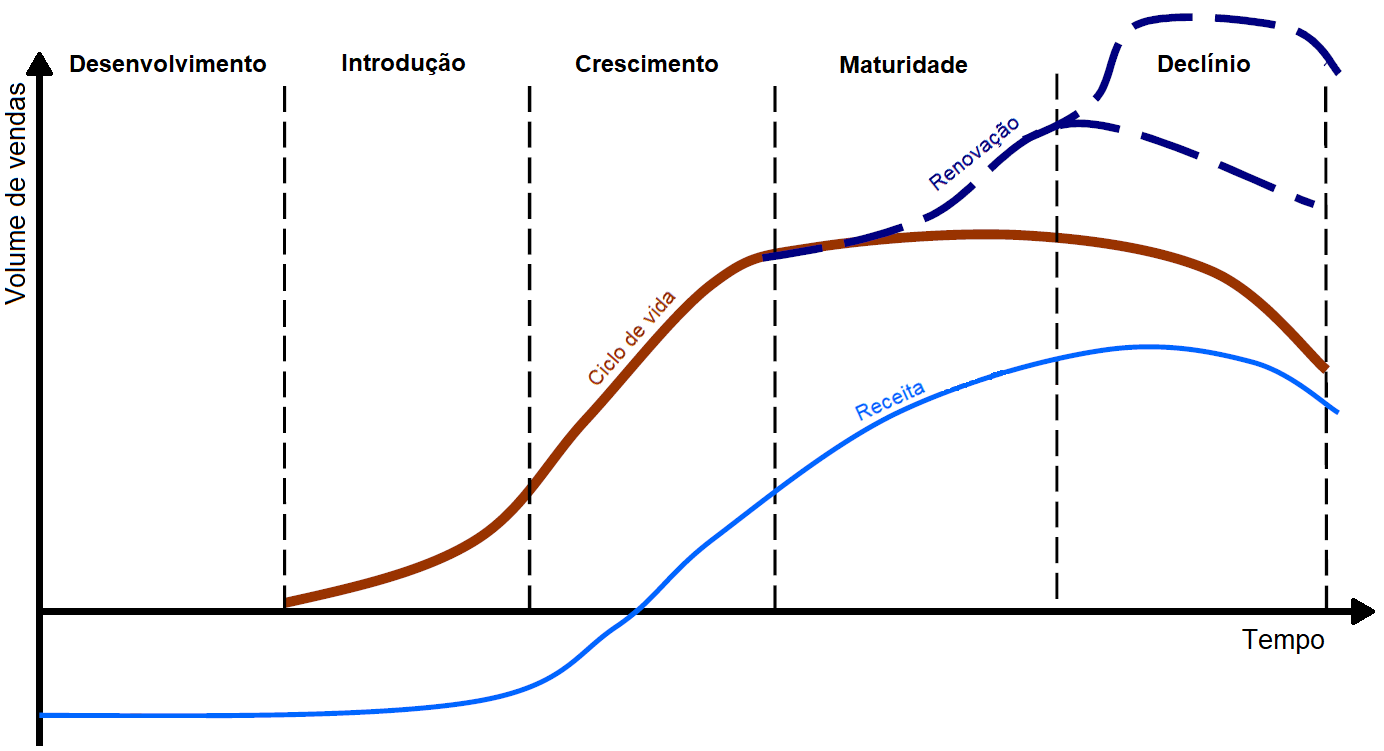
\includegraphics[width=1\textwidth]{life-cycle-extension.png}
		\label{fig:life-cycle-extension}
		\source{\citeonline{liu2010marketingrisk} (adaptado).}
	\end{figure}
	
	Novas propostas de modificações de processos industriais aparecem como formas de se agregar mais valor ao produto/serviço considerando os ciclos de vida do produto cada vez mais curtos. Duas linhas de pesquisas criadas recentemente buscam trazer soluções para os problemas contemporâneos da indústria, como os listados anteriormente, que são os conceitos de Indústria 4.0 (I4.0) e Memória Digital do Produto (MDP).
	
	I4.0 e a MDP são conceitos altamente correlacionados, porém ainda não amplamente abordados em conjunto na literatura, criando assim uma oportunidade de pesquisa a partir de uma lacuna existente.
	
	
\section{Indústria 4.0}

	A crescente integração das Tecnologias da Informação e Comunicação (TIC) às cadeias de valor industriais criou as bases para a próxima revolução industrial chamada Indústria 4.0 \cite{hermann2016design}. Essa mudança de paradigma na indústria se refere às recentes modificações em relação às tecnologias de manufatura, que passam a proporcionar um alto nível de automação e intercâmbio de informações entre equipamentos, produtos e demais atores em um ambiente de manufatura \cite{lasi2014industryfour}. 
	
	O nome Indústria 4.0 (I4.0) se dá ao fato de ser considerada a quarta maior revolução com relação à tecnologia de produção industrial, sendo as ``revoluções industriais'' consideradas evoluções tecnológicas que levaram a grandes mudanças no paradigma de produção, tal histórico de revoluções no campo da indústria é ilustrado na Figura \ref{fig:i4}.

	\begin{figure}[H]
		\centering
		\caption{As revoluções industriais.}
		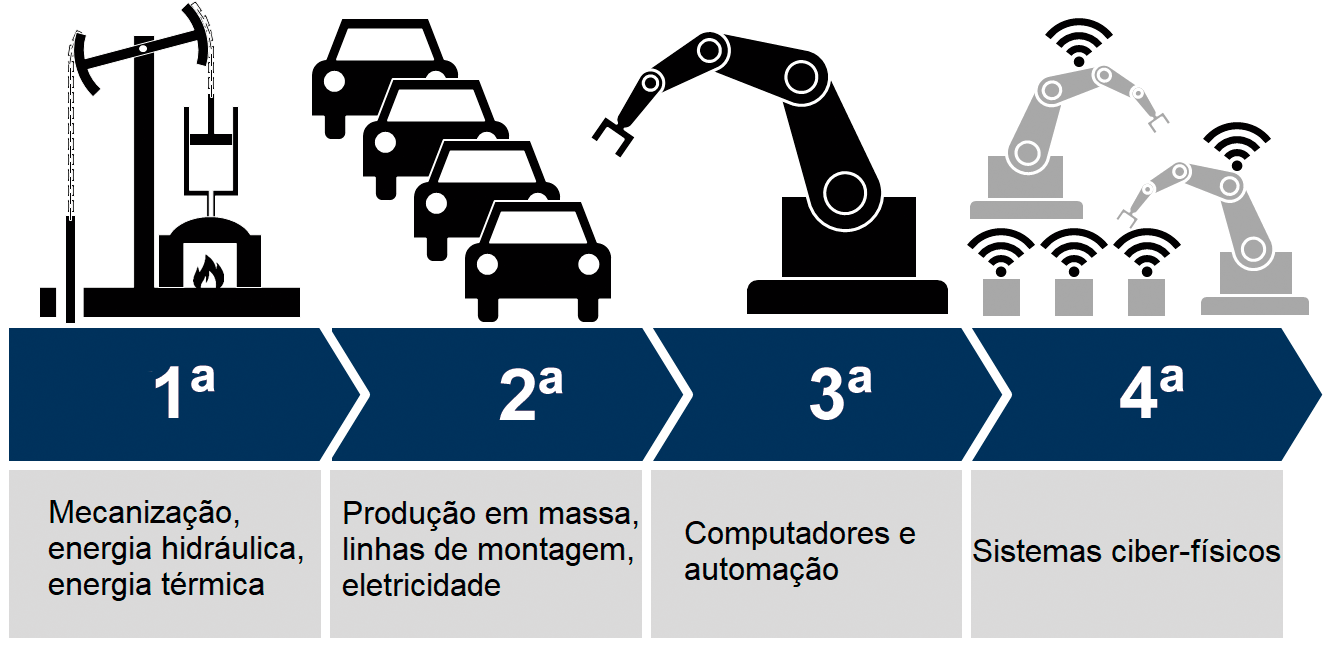
\includegraphics[width=1\textwidth]{i4.png}
		\label{fig:i4}
		\source{\citeonline{lasi2014industryfour} (adaptado).}
	\end{figure}

	Tais modificações na indústria são essenciais devido às novas necessidades da própria indústria e de mudança de padrões de consumo do mercado. Isto acarreta mudanças no cenário operacional destas indústrias. Algumas das causas dessas mudanças operacionais são \cite{lasi2014industryfour}:
	
	\begin{itemize}

		\item Períodos de desenvolvimento curtos: Os períodos de desenvolvimento e inovação de produtos estão sendo reduzidos. A alta capacidade de inovação está se tornando um fator de sucesso para muitas empresas (\textit{Time to market});
		
		\item Individualização sob demanda: Os compradores passam a definir as condições de compra. Essa tendência leva a uma crescente individualização de produtos com características altamente personalizadas e, em casos extremos, a produtos individuais;
		
		\item Flexibilidade: Devido à individualização sob demanda, novas estruturas e organizações na indústria são essenciais para a fabricação de produtos com alto grau de personalização. É necessária uma maior flexibilidade no desenvolvimento do produto, especialmente na produção;
		
		\item Descentralização: Para lidar com condições específicas de cada produto, são necessários procedimentos mais rápidos de tomada de decisão. Para isso, as hierarquias organizacionais precisam ser reduzidas, dando ao produto maior independência sobre seu próprio processo de fabricação;
		
		\item Eficiência de recursos: A maior eficiência sobre o uso dos recursos sempre é algo desejável, porém sua importância se intensifica com as tendências de aumento dos preços dos recursos, bem como a mudança social no contexto de aspectos ecológicos. Isto exige um foco mais intensivo em sustentabilidade, o que decorre em uma maior racionalidade (ou eficiência) na utilização dos recursos.

	\end{itemize}

	Embora o termo I4.0 seja bastante comum na discussão tecnológica atual, muitas empresas, centros de pesquisa e universidades não mantém uma definição comum sobre o assunto. Segundo \citeonline{hermann2016design} e com base em uma revisão de literatura feita pelo mesmo autor, a I4.0 é identificada por quatro princípios de projeto para sua implementação, conforme listados na Tabela \ref{tab:principios-i4}.


	\begin{table}[H]
		\centering
		\caption{Princípios para implantação da I4.0 baseados em \citeonline{hermann2016design}.}
		\resizebox{\textwidth}{!}{%
		\begin{tabular}{|p{1.3in}|p{4in}|}
			\hline
			\textbf{Princípio} & \textbf{Descrição}                                                                                                                                 \\ \hline
			Interoperabilidade & Capacidade das coisas (máquinas, dispositivos, sensores, pessoas, etc) de comunicarem entre si dentro de um sistema por meio de padrões definidos. \\
			\hline
			Transparência de informação &
				Tornar acessíveis informações úteis para os demais dispositivos conectados à rede. Informações do mundo virtual como documentos eletrônicos, desenhos, modelos de simulação; e informações sobre o mundo real, como posição, dados de sensores de temperatura, vibração, etc. \\
			\hline
			Descentralização de decisões &
				Tomada de decisões baseadas nas informações coletados pelo próprio dispositivo da ao dispositivo autonomia para decidir qual será sua próxima função/operação. Desta forma, um planejamento ou controle central de processos produtivos não se faz essencial e o sistema de produção se torna menos hierarquizado. \\
			\hline
			Assistência técnica &
				Devido à complexidade da produção, com redes complexas e tomada decisões descentralizadas, os seres humanos precisam ser auxiliados por sistemas de assistência, de forma a dar compreensibilidade ao processo e às tomadas de decisão necessárias. Os sistemas de assistência devem agregar e tornar visualizável as informações de maneira compreensível. \\ \hline
		\end{tabular}%
		}
		\label{tab:principios-i4}
		\source{O autor.}
	\end{table}




	Os princípios elencados na Tabela \ref{tab:principios-i4} são diretrizes para o desenvolvimento de arquiteturas para a I4.0. As arquiteturas surgem com a necessidade de se definir padrões para a implantação de um sistema. Por ser um assunto novo, as arquiteturas de sistemas produtivos voltadas para a quarta revolução industrial também se encontram em estágio inicial \cite{pisching2018arquitetura}. Hoje, o mais consolidado modelo de arquitetura para a Indústria 4.0 é o RAMI4.0 (Modelo de Arquitetura de Referência para a Indústria 4.0). Esse modelo de arquitetura foi apresentado na feira industrial de Hanôver na Alemanha em abril de 2015.
	
	O RAMI4.0 requer uma representação tridimensional, conforme a Figura \ref{fig:rami4}. Nos três eixos do RAMI4.0 são descritos os níveis hierárquicos de uma fábrica ligada em rede através da Internet (Eixo Níveis Hierárquicos), a representação de arquitetura dos componentes I4.0 (Eixo Camadas) e o ciclo de vida de instalações e de produtos (Eixo Ciclo de Vida e Cadeia de Valor).
	
	\begin{figure}[H]
		\centering
		\caption{Representação do RAMI4.0.}
		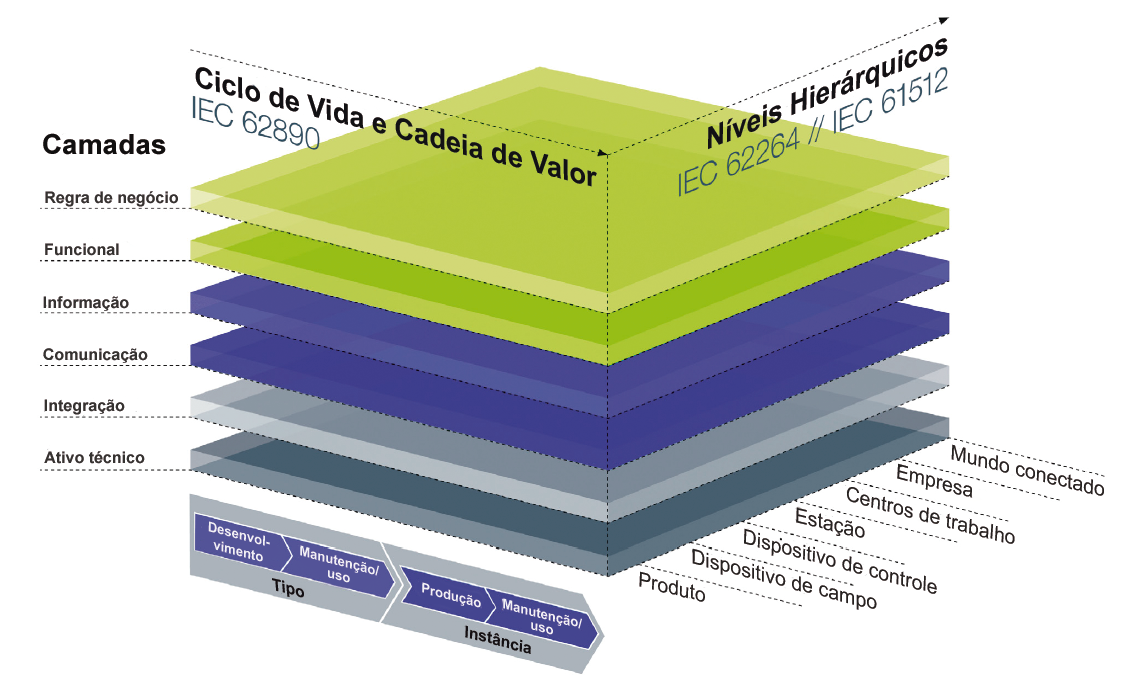
\includegraphics[width=1\textwidth]{rami4.png}
		\label{fig:rami4}
		\source{\citeonline{adolphs2015rami} (adaptado).}
	\end{figure}

	O RAMI4.0, como um modelo de referência, é um elemento para padronização do projeto e implantação de aplicações em I4.0. O RAMI4.0 é uma padronização de linguagem e deve ser aceito e usados por todos os participantes para protótipo, desenvolvimento e validação.

\section{Memória Digital do Produto}

	O termo ``Memória Digital do Produto'' (MDP) surgiu pela primeira vez em 2007 por meio de um boletim de notícias de tecnologia de uma empresa alemã fabricante de conectores elétricos e eletrônicos \cite{wahlster2007digitalmemory}. À época, o termo foi tratado com analogia a um diário, que mantinha todas as informações do produto ao longo de seu ciclo de vida.

	Hoje, o conceito na literatura se refere a sistemas que permitem a coleta de dados em todas as fases do ciclo de vida do produto para a distribuição e/ou análise. Os dados de interesse do produto podem ser relativos a qualquer fase do produto ao longo de sua cadeia de valor, o que abrange dados de produção individual, de montagem, de distribuição, de uso por parte do consumidor, etc. A Figura \ref{fig:MDP-ideia} ilustra o conceito de MDP.
	 
	\begin{figure}[H]
		\centering
		\caption{Coleta de dados do produto ao longo da cadeia de valores.}
		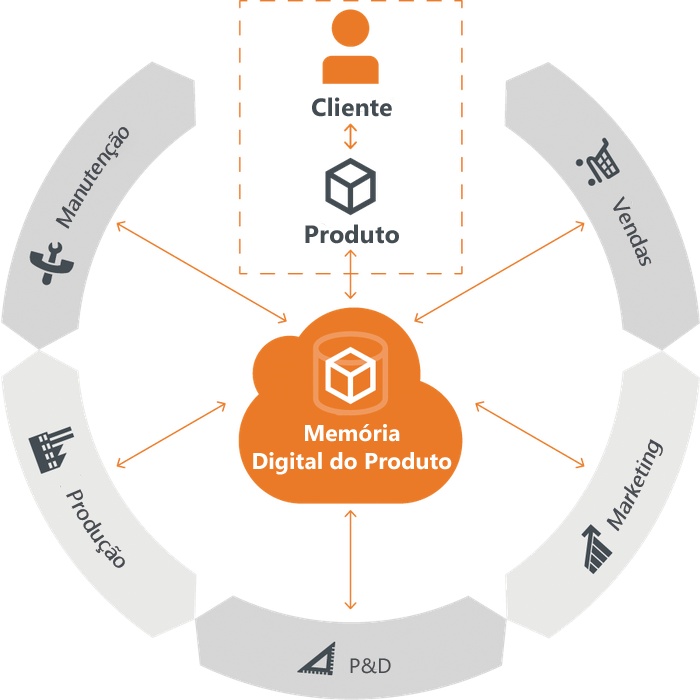
\includegraphics[width=0.6\textwidth]{MDP-ideia.png}
		\label{fig:MDP-ideia}
		\source{\citeonline{zuhlke2020digitalmemory} (adaptado).}
	\end{figure}

	Sua relevância está no fato da tendência de produtos novos apresentarem ciclos de vida cada vez mais curtos e devido ao fato das cadeias de suprimentos apresentarem redes cada vez mais complexas, com múltiplos fornecedores e clientes. Com isso, a MDP manteria registros digitais do ciclo de vida dos produtos, faria o monitoramento constante do seu estado atual e realizaria o rastreamento de sua posição. Segundo \citeonline{wahlster2007digitalmemory}, o acesso a essas informações pelas partes interessadas seria de vital importância na competitividade de empresa produtoras e de comércio, além de abrir novas proteções em relação à pirataria.
	
	A implementação de uma memória com informações sobre produto ao longo de sua cadeia de valores é importante, pois torna possível acessar e utilizar informações do mundo real providenciada por diferentes fontes ao longo da cadeia de suprimentos para o potencial benefício das partes interessadas naquele produto \cite{brandherm2011productmemory}, como, por exemplo, fabricantes, transportadores, varejistas e consumidores. 
	
\section{Interrelação entre I4.0 e MDP}

 	Ambos os conceitos de I4.0 e MDP são conceitos recentes, surgidos em 2011 \cite{kagermann2011industrie} e 2007 \cite{wahlster2007digitalmemory}, respectivamente . A área multidisciplinar de estudo envolvendo MDP e I4.0 surgira em 2013 com o projeto SemProM \cite{wahlster2013semprom}, porém ainda quando I4.0 era um conceito abrangente e sem diretrizes concretas para sua implementação, que ocorreria em 2013 por meio do documento de recomendações para implementação da iniciativa estratégia Industrie 4.0 \cite{kagermann2013recommendations}; e sem a criação do modelo de arquitetura de referência para Indústria 4.0 (RAMI4.0), que seria divulgada em 2015 por meio do documento entitulado ``RAMI4.0'', divulgado por um periódico alemão \cite{hankel2015rami}.
 	
 	 Alguns outros estudos como \citeonline{lasi2014industryfour} citam MDP como oportunidade de estudo e aplicação dentro da I4.0, outros como \citeonline{weyer2015standardization} e \citeonline{paelke2014augmented} implementam sistemas práticos envolvendo ambos os conceitos, porém sem considerações sobre cadeia de valor.
 	
	Há estudos na área multidisciplinar de I4.0 e MDP, principalmente no meio acadêmico, empresarial e governamental alemão pelo fato de esses conceitos terem surgido na Alemanha. Porém nenhum trabalho até o presente momento relaciona o modelo de arquitetura de referência para a I4.0 (RAMI4.0) com a MDP, o que aponta uma lacuna de conhecimento dentro de I4.0 a ser explorada.
	
	Estudos sobre o RAMI4.0 são importantes no sentido de padronizar a implementação da I4.0 em empresas de diferentes negócios, garantindo assim a interoperabilidade dos serviços. O eixo ``Ciclo de Vida e Cadeia de Valor'' apresenta diretrizes para o correto planejamento da vida de um produto e sugere cenários para criação de valor perceptível ao produto/serviço. Integrar o conceito de MDP ao RAMI4.0, especificamente ao eixo de ``Ciclo de Vida e Cadeia de Valor'', enriquece o nível de discussão sobre essa arquitetura de referência e dá mais robustez ao modelo para uma futura adoção generalizada por parte de empresas por todo o mundo.
	
	A ``Plattform Industrie 4.0'' é uma das principais redes mundiais de discussão sobre I4.0 \cite{kagermann2013recommendations, acatech2014plattform, germany2019plattform}. O Conselho de Pesquisa da Plattform Industrie 4.0 é o comitê consultivo estratégico da Plattform Industrie 4.0 e identifica necessidades de pesquisa e ações em torno da I4.0. O comitê identificou e definiu quatro temas-chave de abordagens no setor tecnológico, econômico, metodológico e social/legal para se implementar com sucesso a I4.0 \cite{hirsch-kreinsen2019keythemes}, conforme mostrado na Figura \ref{fig:keythemes-i4}. Isso significa que os tópicos elencados são temas com alto potencial para a otimização de rotinas e processos de produção existentes no cenário de I4.0.
	
	\begin{figure}[H]
		\centering
		\caption{Temas-chave de pesquisa e desenvolvimento em I4.0.}
		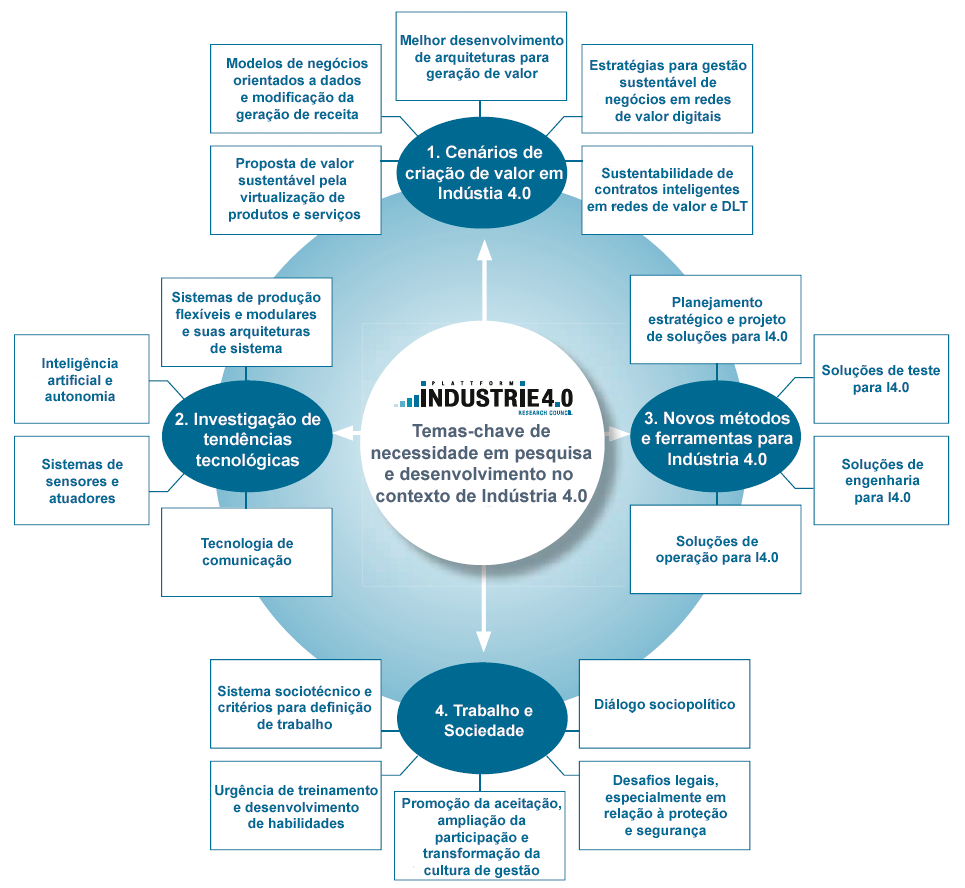
\includegraphics[width=1\textwidth]{keythemes-i4.png}
		\label{fig:keythemes-i4}
		\source{\citeonline{hirsch-kreinsen2019keythemes}.}
	\end{figure}

	Dentre os temas elencados na Figura \ref{fig:keythemes-i4}, destacam-se os subitens relacionados ao tópico ``Cenários de criação de valor em Indústria 4.0'' por estarem altamente relacionados ao RAMI4.0 e ao conceito de geração de valor por meio da MDP. O desenvolvimento de arquiteturas para geração de valor e a criação de negócios orientados a dados são temas de grande oportunidade dentro do cenário de I4.0, especialmente se considerando os métodos quantitativos de \textit{Business Intelligence} e de análise de dados já estabelecidos.
	

\section{Objetivos da pesquisa}

	O objetivo do trabalho de pesquisa é a investigação da integração do conceito de MDP ao RAMI4.0, especificamente ao eixo de ``Ciclo de Vida e Cadeia de Valor'', de forma a se aperfeiçoar a elaboração dessa arquitetura a fim de proporcionar mais robustez ao modelo para uma futura adoção generalizada por parte de empresas por todo o mundo.
	
	Todo o estudo é feito com a proposta de aperfeiçoar o RAMI4.0 no sentido de propiciar o surgimento de novos cenários de criação de valor no contexto de I4.0 e incentivar geração de novos modelos de negócio baseado em dados.
	
	Este plano de pesquisa envolve o estudo de diversos temas relacionados à Indústria 4.0. Os principais itens estão explicitados a seguir. Diversos novos itens são adicionados ao foco de pesquisa à medida que há aprofundamento nos itens abaixo.
	
	\begin{itemize}
		\item Indústria 4.0;
		\item RAMI4.0;
		\item Cadeia de valor;
		\item Ciclo de vida do produto;
		\item Memória digital do produto;
		\item Internet das coisas.
	\end{itemize}
	
	Tais temas são estudados a fim de se analisar o estado da arte atual em I4.0 e a partir disso propor alterações sobre o RAMI4.0 incluindo o conceito de MDP.





























% ----------------------------------------------------------







	
	
	

	
	
	


